\documentclass[journal, 11pt]{IEEEtran}

% *** CITATION PACKAGES ***
%
%\usepackage{cite}https://www.overleaf.com/project/5d8e32cf8b64620001d24060
\usepackage{capt-of}%%To get the caption
\usepackage{gensymb}
\usepackage{graphicx} %package to manage images
\graphicspath{ {./images/} }
\usepackage{wrapfig}

\usepackage{amsmath}
\usepackage{amssymb}
\usepackage{hyperref}
\usepackage{lipsum}

\usepackage[style=ieee]{biblatex}
\DeclareLanguageMapping{english}{english-apa}
\addbibresource{references.bib}
\usepackage[justification=centering]{caption}

\usepackage{setspace}

\usepackage{hhline}


\usepackage{changepage} 

\usepackage{booktabs}
\usepackage{xcolor}

\usepackage{makecell}
\usepackage{graphicx,subcaption}
\usepackage{listings}
\renewcommand\theadfont{}
\DeclareMathOperator{\EX}{\mathbb{E}}% expected value


\usepackage{multicol} 

%\raggedbottom

\begin{document}


\pagenumbering{gobble}
%\clearpage\mbox{} % adds and empty page
%\clearpage
\pagenumbering{arabic}
\setcounter{page}{1}

\title{\LARGE{Flyway: Predicting Foot Traffic in Open Spaces on Campus}}

\author{ ENGR-UH 4560 Machine Learning, Fall 2019\\
\medskip
Nishant Aswani,~\IEEEmembership{nsa325@nyu.edu}
Barkin Simsek,~\IEEEmembership{bs3528@nyu.edu}}% <-this % stops a space


% The paper headers
\markboth{Aswani, Simsek ENGR-UH 4560 Machine Learning, Fall 2019}%
{}

% make the title area
\maketitle

% As a general rule, do not put math, special symbols or citations
% in the abstract or keywords.
% \begin{abstract}


% \end{abstract}

%%%%%%%%%%%%%%%%%%
%% Introduction %%
%%%%%%%%%%%%%%%%%%
\section{Introduction}
\subsection{Motivation}
\IEEEPARstart{P}\lowercase{redicting} traffic is one of the most common timeseries forecasting problems available for tackling. When placed in the context of smart cities, the problem is motivated by the question of "how to enable users to make smarter choices when using transportation networks" \cite{lv2014traffic}. However, this can be broadened to include how smart choices are made for using infrastructure and public spaces in general. \\

\noindent Given that our campus has multiple open spaces for students to study and/or relax, we want to be able to forecast the foot traffic that occurs in the multiple spaces. This could eventually be furthered, and the information organized, to provide a live prediction visualization of foot traffic around campus.

\subsection{Problem Statement}

\noindent Gathering from our previous experience with the New York City (NYC) taxi data set, we had a rough idea on how to approach timeseries data, along with the models and analysis that is carried out on such data. We were able to draw parallels between foot traffic in our project to pickup counts in certain locations in NYC.

%%%%%%%%
% NOTE %
%%%%%%%%
% include info about how we gather the data, why we gather the data that way, and why we get that specific data or those features

\section{Existing Body of Work}

\subsection{Past Projects}

\noindent One of the inspirations of this project was the Waitz application developed by students at University of California San Diego (UCSD) \cite{waitz}. They used Raspberry Pi's, loaded with network monitoring firmware and placed at various locations around their campus, to approximate the number of students within a given area. They did so by logging the Bluetooth and MAC addresses of devices within range of the network sniffing Pis. It is not clear how they tackled the issue of mapping the number of devices to the number of students.\\

% \begingroup
%     \centering
%     \medskip
%     %width=\columnwidth
%     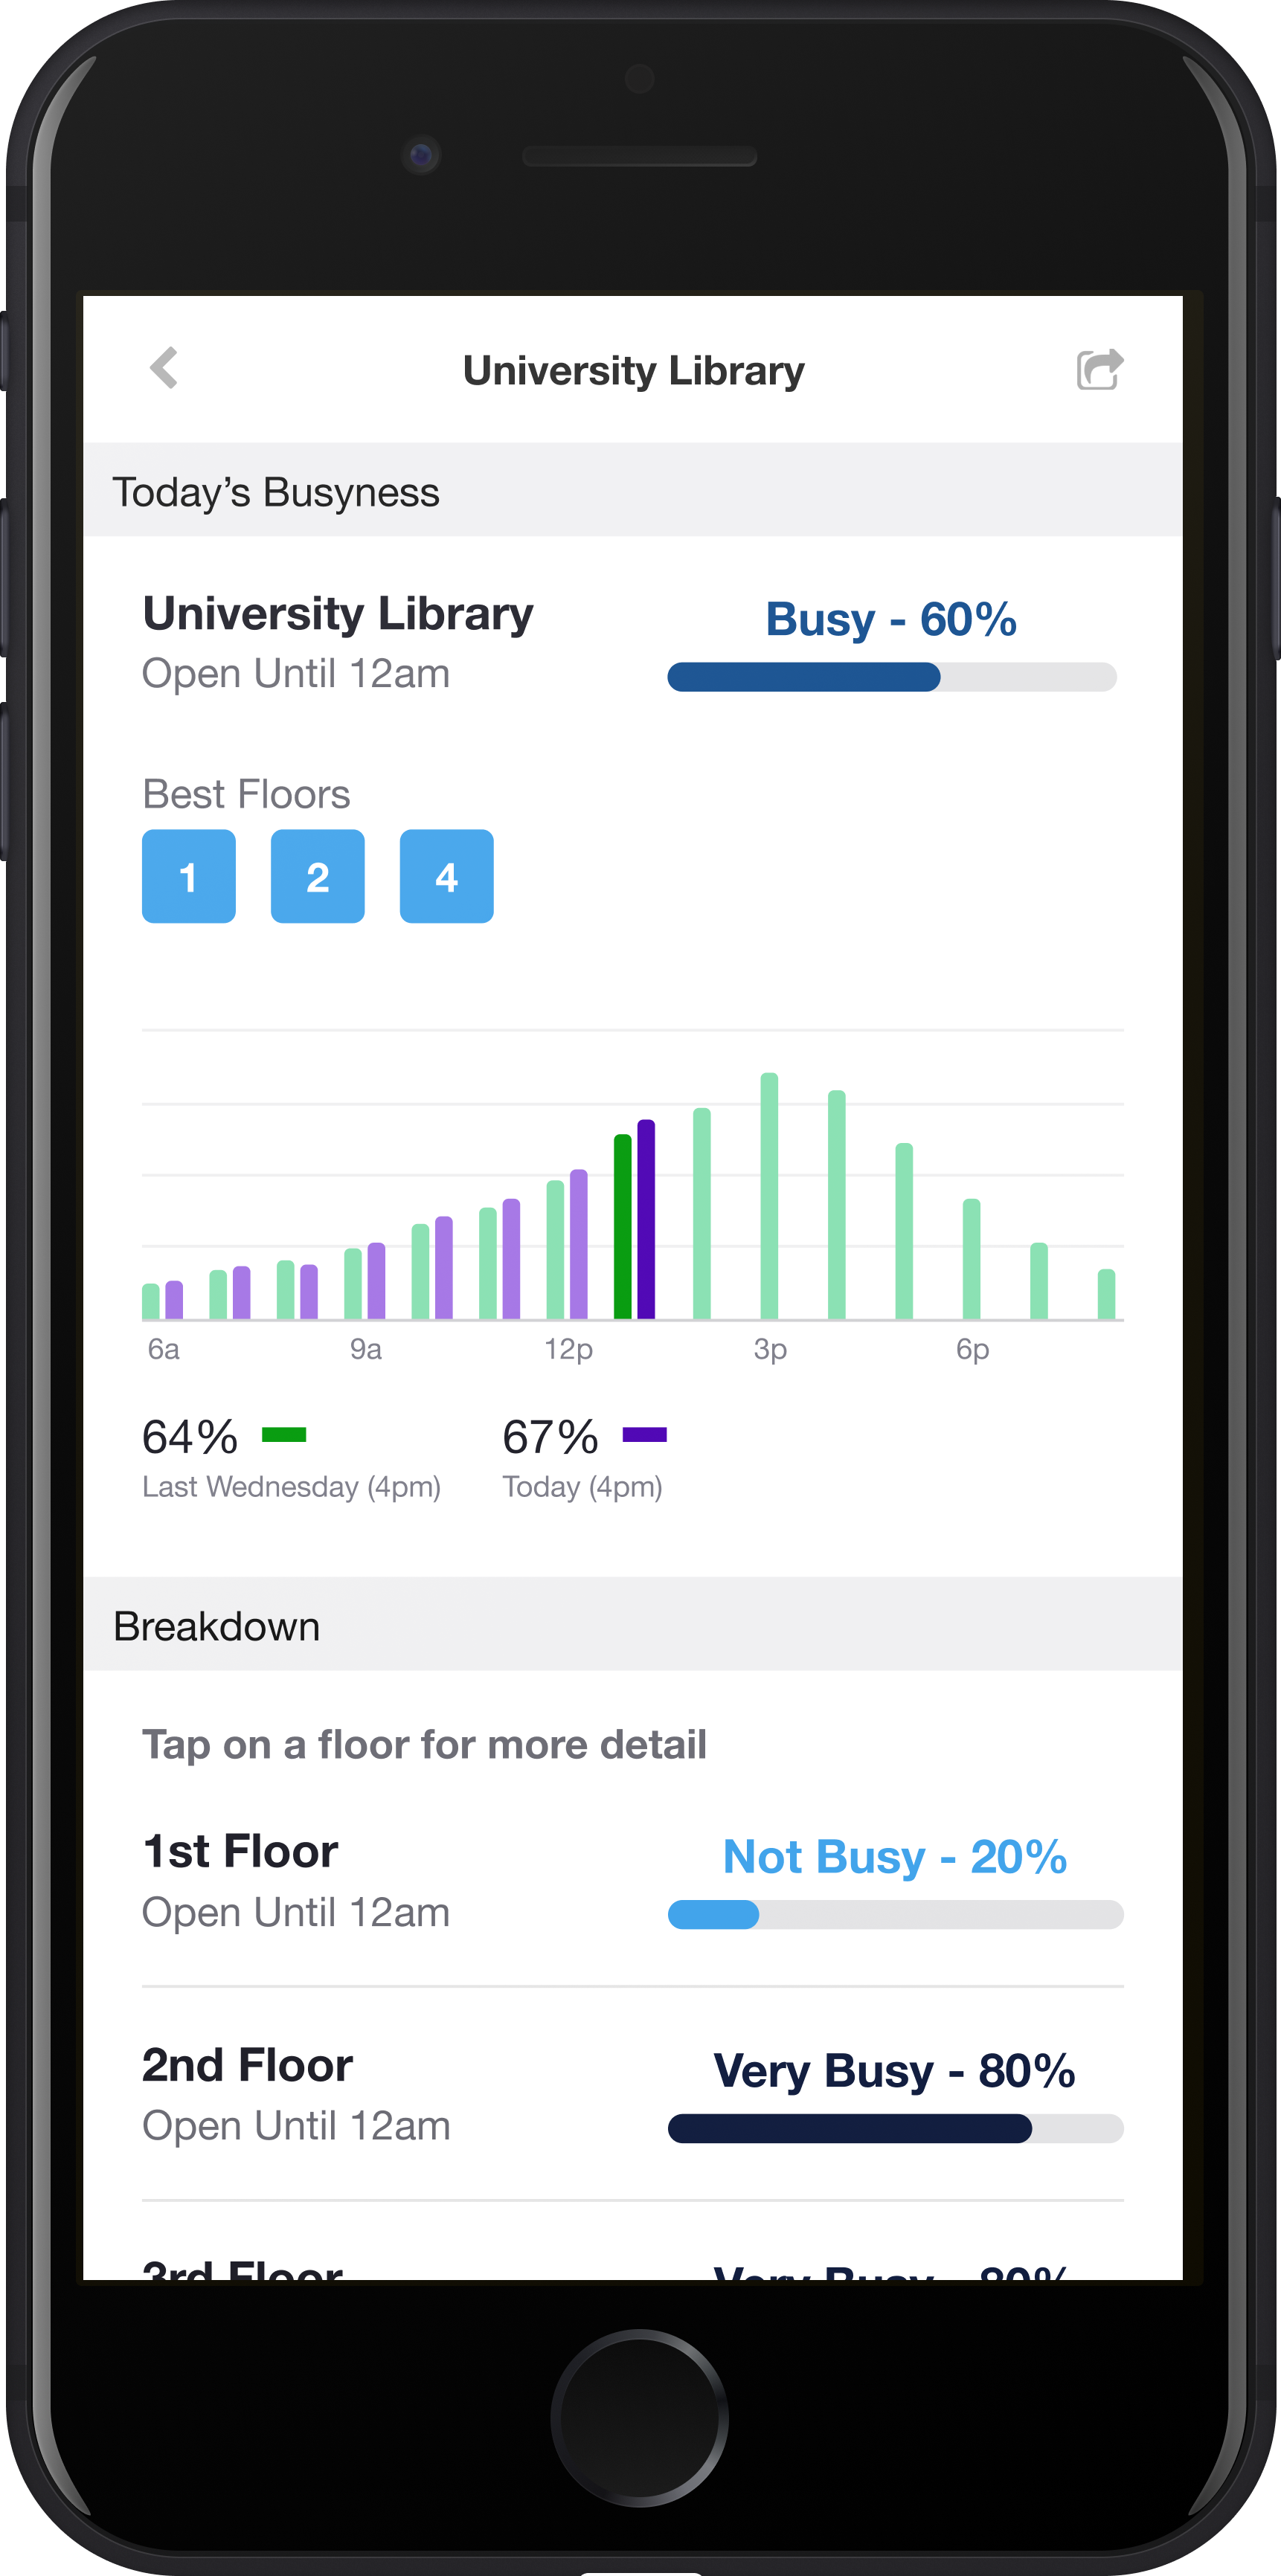
\includegraphics[width=0.4\columnwidth]{./images/waitz.png}
%     \captionof{figure}{Waitz UI}
%     \label{fig:waitz_ui}
%     \medskip
% \endgroup
% \medskip

\noindent However, their application is relatively simple as they did not use this data to forecast the "busyness" of locations or make predictions. Instead, it seems that they focused more on data collection and visualization. As a result, we thought it would be interesting to implement a similar tool for our campus; in the process, we hoped discover if there are any timeseries patterns we can exploit to provide useful information for students.

\subsection{Literature}

\noindent Unsurprisingly, there have been several attempts at using machine learning to determine "crowdedness" or "busyness". One of the benefits of searching through published work was being able to pick up on vocabulary within the field of research, making it easier to find other works. \\

\noindent We found that published work refers to this topic as "occupancy prediction" using "Wifi probing"\cite{wang2018occupancy}. Specifically, the work published by Wang et. al. determined five main characteristics in their occupancy prediction project. They realized their collected data had a "time-series characteristics" \cite{wang2018occupancy}, validating our hypothesis that occupancy is relative to time of day, as well as the idea that past data can feasibly predict future data. While this may be trivial to the overall project, it was a source of confidence for our project as it implied we could successfully build a reasonably performing model. \\

\noindent The researchers implemented an "Markov-based feedback Recurrent Neural
Networks (M-FRNN)" \cite{wang2018occupancy} model as part of their project to predict occupancy

\section{Methodology}
\noindent The methodology for realizing this project has 4 main steps: data collection, data processing, data analysis, and user interface. Data collection is the lowest level in the process and it is achieved by using ARM based Raspberry Pi Zero computers since they have builtin bluetooth and WIFI chips. Besides having the WIFI chip as an hardware, the WIFI chip itself should be supporting the "monitoring" mode for monitoring the wireless traffic. The WIFI chip of Raspberry Pi Zero also has this monitoring feature that enables the data collection for the project.

\begingroup
    \center
    \medskip
    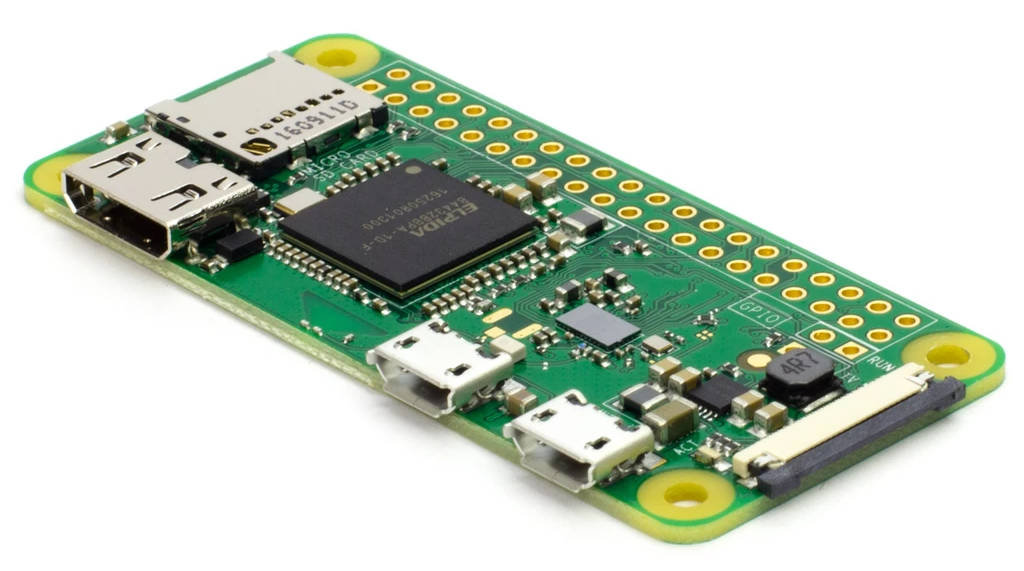
\includegraphics[width=0.6\columnwidth]{report/interim_report/images/raspi.png}
    \captionof{figure}{Raspberry Pi Zero used for data collection}
    \label{fig:raspi}
    \medskip
\endgroup

\noindent The  Raspberry Pi Zero computer is running a special version of the Linux operating system and this also helps us with the data collection since Linux natively supports the \texttt{dumpcap} tool, which was used to collect the data packages in the air. Further details related to the \texttt{dumpcap} network traffic dump tool can be found  \href{https://linux.die.net/man/1/dumpcap}{here}.\\

\noindent When a WIFI chip is in the monitoring mode it is not capable of collecting private data since WIFI traffic between devices and the routers are already encrypted with some sort of password protection. That being said, we can still get various data regarding the source and destination of the data packages. These non-private information is enough for our project since we want to be able to approximately count the number devices and people in a space rather than spying on personal data. The following are the data fields that can be collected while monitoring WIFI signals in the monitoring mode:

\begin{itemize}
    \item frame.number
    \item frame.time
    \item wlan.addr
    \item wlan.ta
    \item wlan.ra
    \item wlan.sa
    \item wlan.da
    \item wlan.bssid
    \item wlan.fc.type
    \item wlan.fc.type\_subtype
    \item radiotap.channel.freq
    \item radiotap.datarate
    \item radiotap.dbm\_antsignal
\end{itemize}

\noindent 


\subsection{Feasibility}


%%%%%%%%
% NOTE %
%%%%%%%%
% include information about some nuances we need to think about or we can extract. For example, do we have to worry about someone "passing by" if their MAC address was available for just a small bit of time. 




\subsection{Applicability to Solving the Problem}


%%%%%%%%%%%%%%%%%%%%%%%%%
%% Experimental Method %%
%%%%%%%%%%%%%%%%%%%%%%%%%

%%%%%%%%%%%%%
%% Results %%
%%%%%%%%%%%%%

%%%%%%%%%%%%%%%%
%% Discussion %%
%%%%%%%%%%%%%%%%

\printbibliography

\end{document}

%%%%%%%%%%%%%%%
%% Equations %%
%%%%%%%%%%%%%%%

% \begin{equation}
%     \begin{split}
%         X &\texttt{\char`\~} Poisson(\lambda) \\
%         \\
%         P(X=k) &= \frac{\lambda^k e^{-\lambda}}{k!} \\
%         \\
%         \EX(k) &= e^{-\lambda}\sum_{k=1}^{\infty} \frac{\lambda^n}{(n-1)!}\\
%         \\
%         &= e^{-\lambda}\lambda\sum_{k=1}^{\infty} \frac{\lambda^{k-1}}{(k-1)!}\\
%         \\
%         &= e^{-\lambda}\lambda\sum_{n=0}^{\infty} \frac{\lambda^{n}}{(n)!}\\
%         \\
%         &= e^{-\lambda}\lambda e^{\lambda} = \lambda\\
%     \end{split}
%     \label{eq:mutual}
% \end{equation}

% \noindent Hence, we know that the $\lambda$ parameter can be approximated as the mean degree.

% \begin{equation}
%     \begin{split}
%         \lambda = \frac{\sum_{i=1}^{n}D_i}{n}
%     \end{split}
%     \label{eq:poisson_distribution}
% \end{equation}

%%%%%%%%%%%
%% Table %%
%%%%%%%%%%%

% \begingroup
%     \medskip
%     \centering
%     \def\arraystretch{1.5}
%         \begin{tabular}{lcc}
%             \toprule
%             & Random Network & Scale-Free Network \\
%             \midrule
%             Avg. of Avg. Degree    & 3.9988    &  4.0035   \\
%             Var. of Avg. Degree    & 7.6800$\times 10^{-7}$ & 3.1156$\times 10^{-6}$  \\
%             Avg. of Avg. Distance  & 5.5694 & 5.0935    \\
%             Var. of Avg. Distance  & 1.5507 & 0.5377   \\
%             \bottomrule
%         \end{tabular}
%     \captionof{table}{Statistics of fifty runs where \\ n = 5,000, e = 10,000}
%     \label{table:fifty_runs}
%     \medskip
% \endgroup
